\subsection{Space Confinement}

Since our drone could potentially move in unexpected ways whilst dancing, we confined it to move only in an allowable volume of space. This space is defined vertically by an altitude limit, and horizontally by an area on the ground, marked by roundels

\subsubsection{Vertical Limit}

We have two measures for imposing an altitude limit. The first is an ``absolute" limit where we manually configure the drone's internal altitude limit to (-----FIND EXACT NUMBER----) cm above the ground. Should the drone reach this altitude, the drone will stop moving, land, and end the program, thus preventing the drone from flying into the ceiling. Realistically, we don't want the drone to stop and land in the middle of a dance routine, so we implemented a second ``soft" limit where we continually track altitude by receiving and reading the drone's navigation data, and if the drone reaches an altitude of (-----FIND EXACT NUMBER ----) cm, our program will instruct the drone to move down for a short duration (1s) (SHOULD I FIX THIS IN THE CODE TO 2s????) and then continue to dance from where it should now be in the routine, after accounting for the 1s delay where the drone was moving down (AGAIN, CHANGE??).

\subsubsection{Horizontal Limit}

For the horizontal limit, we configured the drone to use the ground-facing camera to detect a roundel target. When a roundel target is detected, the program will take the drone's relative orientation then calculate the necessary x- and y- directions for the drone to move away from the roundel without rotation

The ground camera of the AR Drone 2.0 has a 90� field of view.

\begin{figure}[H]
      \centering
      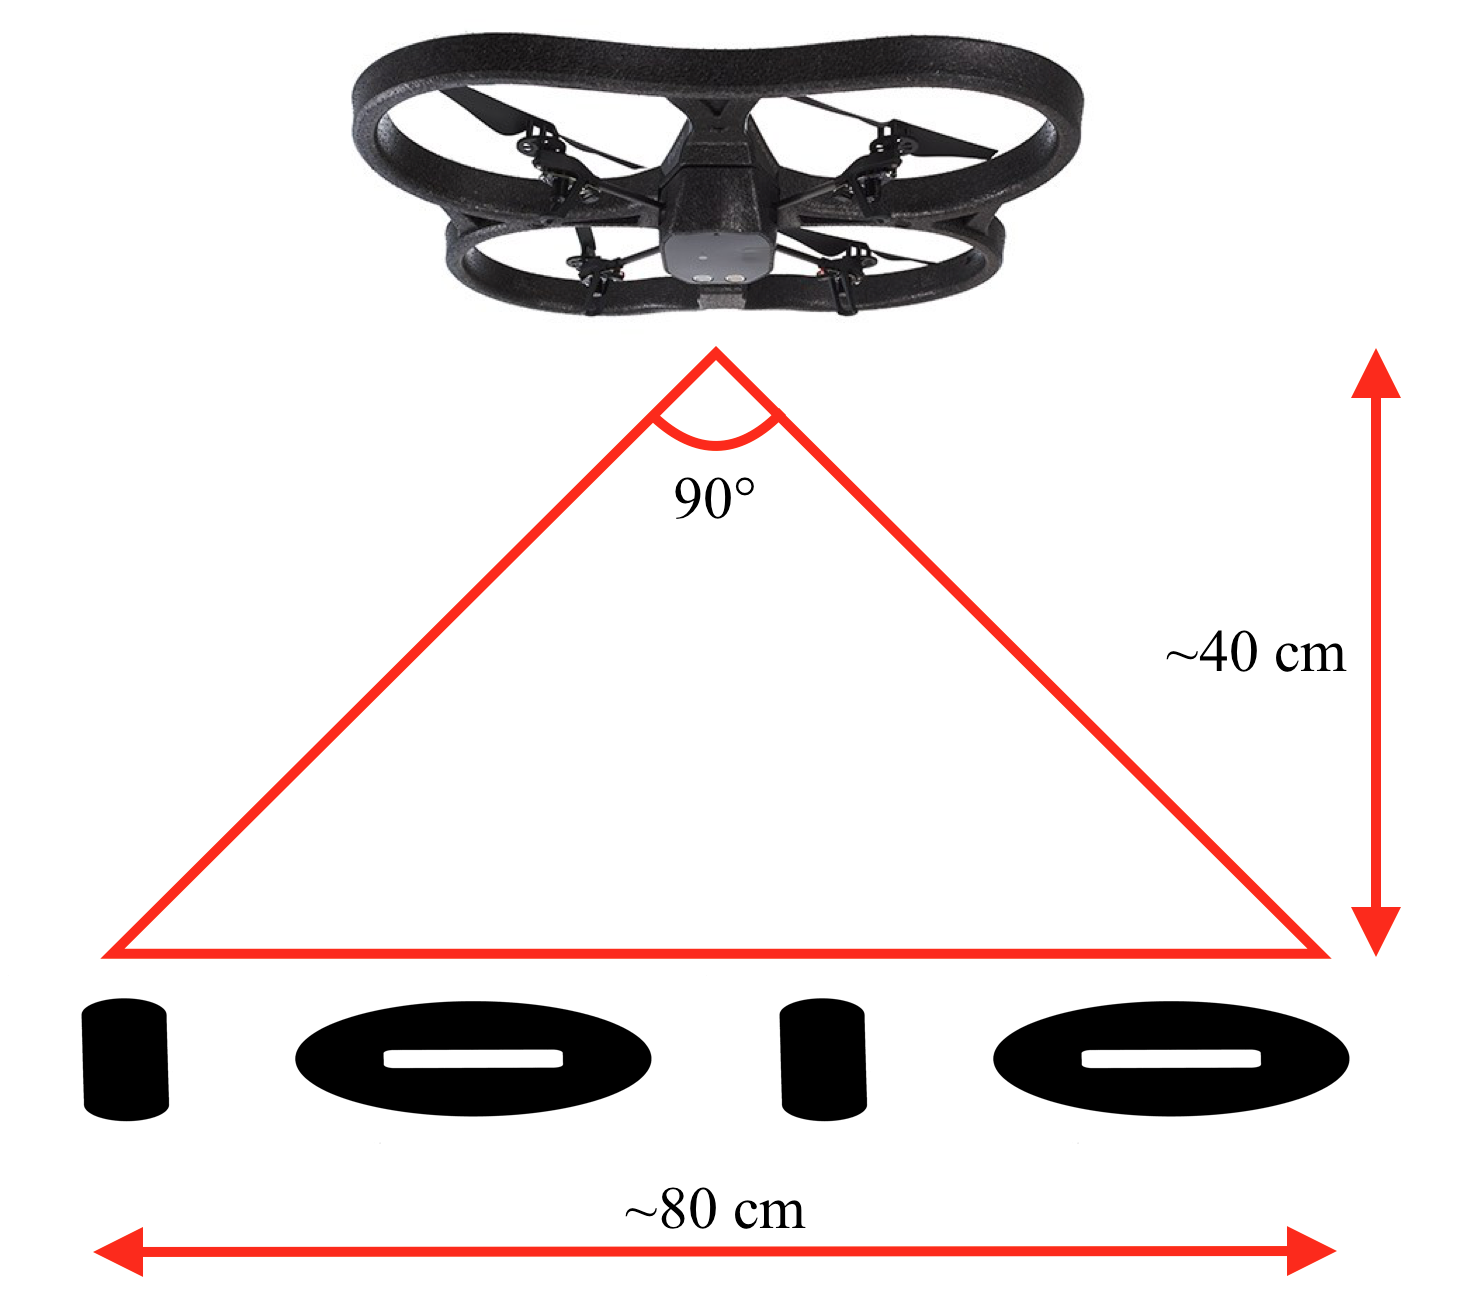
\includegraphics[width=0.8\linewidth]{3d-drone-fov.png}
      \caption{Roundel detection requirements}
\end{figure}